\chapter{The PACE Architecture}
\label{ch:pace}

This chapter describes PACE (Procedural Abstractions for Communicating Efficiently)~\cite{thomas_pace_2025}, the neuro-symbolic architecture this thesis extends. The description follows the methodology of the original paper, organised around the three phases that define the training loop of PACE: Selection, Communication, and Abstraction.

The chapter is organised as follows. Section~\ref{sec:pace-setup} presents the architect-builder game as a concrete setup, establishing the vocabulary (grid, action, primitive, program, scene, message) used throughout the rest of the thesis. Section~\ref{sec:pace-overview} gives a high-level overview of the three phases. Sections~\ref{sec:pace-selection},~\ref{sec:pace-communication}, and~\ref{sec:pace-abstraction} describe the three phases in detail. Section~\ref{sec:pace-training-loop} shows how the three phases fit together in the training loop. Section~\ref{sec:pace-extensions} isolates the two changes this thesis introduces.

\section{The Architect-Builder Game}
\label{sec:pace-setup}

PACE is trained on a specific instance of a collaborative game, the architect-builder game introduced by McCarthy et al.~\cite{mccarthy_learning_2021} and described in Section~\ref{sec:bg-mccarthy-pace-thesis}. In the version PACE uses, the game plays out as follows.

The world is a 9$\times$9 \textbf{grid} of empty cells. There are two \textbf{primitive} building blocks that can be placed on the grid: a horizontal block covering two adjacent cells in a row (denoted $a_{\text{horiz}}$), and a vertical block covering two adjacent cells in a column (denoted $a_{\text{vert}}$). An \textbf{action} $a_i$ consists of choosing one of these two primitives together with a \textbf{position} on the grid, which specifies the column at which the block is dropped; the row is determined automatically by physics (the block falls until it either lands on the floor or on top of a previous block). A \textbf{program} $p$ is a sequence of actions $p = [a_1, a_2, \ldots, a_\ell]$ that, when executed sequentially on an empty grid, produces a specific configuration of blocks called a \textbf{scene}.

Each training \textbf{scene} depicts two shapes placed side by side on the 9$\times$9 grid (Figure 3.1). Each shape is a compact configuration of blocks that resembles a letter of the English alphabet (see Section~\ref{sec:framework-shape-dataset} for the specific list of shapes used). The full dataset contains 961 such scenes, corresponding to all ordered pairs of the 31 shapes. This dataset is split into 930 training scenes and 31 test scenes.

\begin{figure}[htbp]
    \centering
    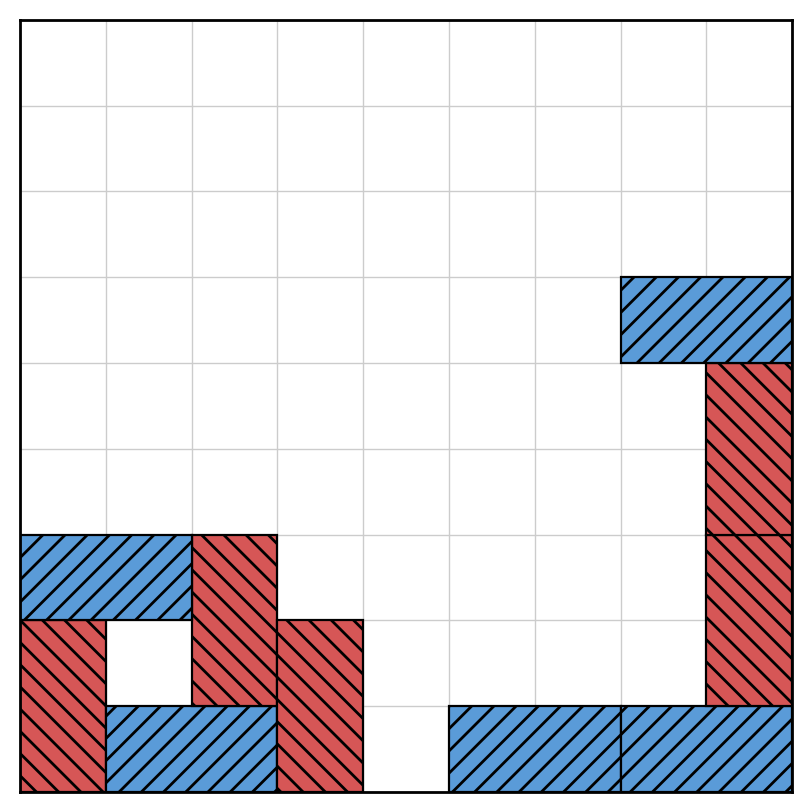
\includegraphics[width=0.35\textwidth]{images/pair.png}
    \caption{Example of a scene from the PACE dataset, showing the pair \texttt{lower\_a upper\_j}. Two shapes are placed adjacent to each other on a 9$\times$9 grid. Blocks placed by horizontal primitive actions are shown in blue; blocks placed by vertical primitive actions are shown in red. The full dataset consists of $31 \times 31 = 961$ such scenes.}
    \label{fig:example-scene}
\end{figure}


The game is played by two agents. The \textbf{architect} sees the target scene and must guide the \textbf{builder}, who cannot see the target, in reconstructing it. The architect does this by selecting a program $p$ and communicating each of its actions $a_i$ to the builder one at a time. The builder's task is to interpret each action and update its internal state of the grid so that after all actions have been communicated, the builder's grid matches the target scene. Throughout the rest of this thesis we refer to these two agents as the \textbf{speaker} and \textbf{listener} respectively, following the broader emergent communication terminology and consistently with the terminology introduced in Chapter~\ref{ch:background}.

Two aspects of this setup are worth stressing. First, PACE does not communicate a whole scene at once: the game unfolds one action at a time, with the speaker producing a fresh message for each action, and the listener updating its grid state after each message. Second, the vocabulary the speaker uses is not fixed at the start of training. Initially the speaker has only two symbols in its lexicon $\mathcal{A}$: those corresponding to the two primitives. Over the course of training, PACE introduces new symbols into $\mathcal{A}$, each representing a reusable sub-sequence of primitives, allowing the same scene to be described with progressively shorter programs. These new symbols are called \textbf{abstractions}.

\section{Overview of the Three Phases}
\label{sec:pace-overview}

PACE decomposes training into three phases that repeat cyclically: \textbf{Selection}, \textbf{Communication}, and \textbf{Abstraction}, illustrated in Figure~\ref{fig:pace-phases}. Each phase corresponds to a different decision the system needs to make.

The Selection phase decides, for each training scene, which of the available programs to communicate. At the start of training there is only one program per scene, so no decision is needed; but as abstractions are introduced, each scene accumulates alternative programs that use the new abstractions in place of some of their primitives, and a choice must be made among them. This choice is handled by a bandit that trades off program length against communicative accuracy.

The Communication phase runs the actual signalling between speaker and listener. For each action in each selected program, the speaker produces a discrete message via a neural policy, and the listener updates its grid state based on that message together with its current state. Both agents are trained end-to-end via gradient descent on a reconstruction loss.

The Abstraction phase introduces one new abstraction into the vocabulary $\mathcal{A}$. It looks at all the sub-sequences of primitives that appear in the current pool of programs, scores them using an MDL-inspired criterion (Section~\ref{sec:bg-mdl}), and selects the one whose introduction would compress the programs the most. Once the new abstraction is added, every program that contains its underlying sub-sequence gains a shorter alternative version that uses the abstraction.

\begin{figure}[htbp]
    \centering
    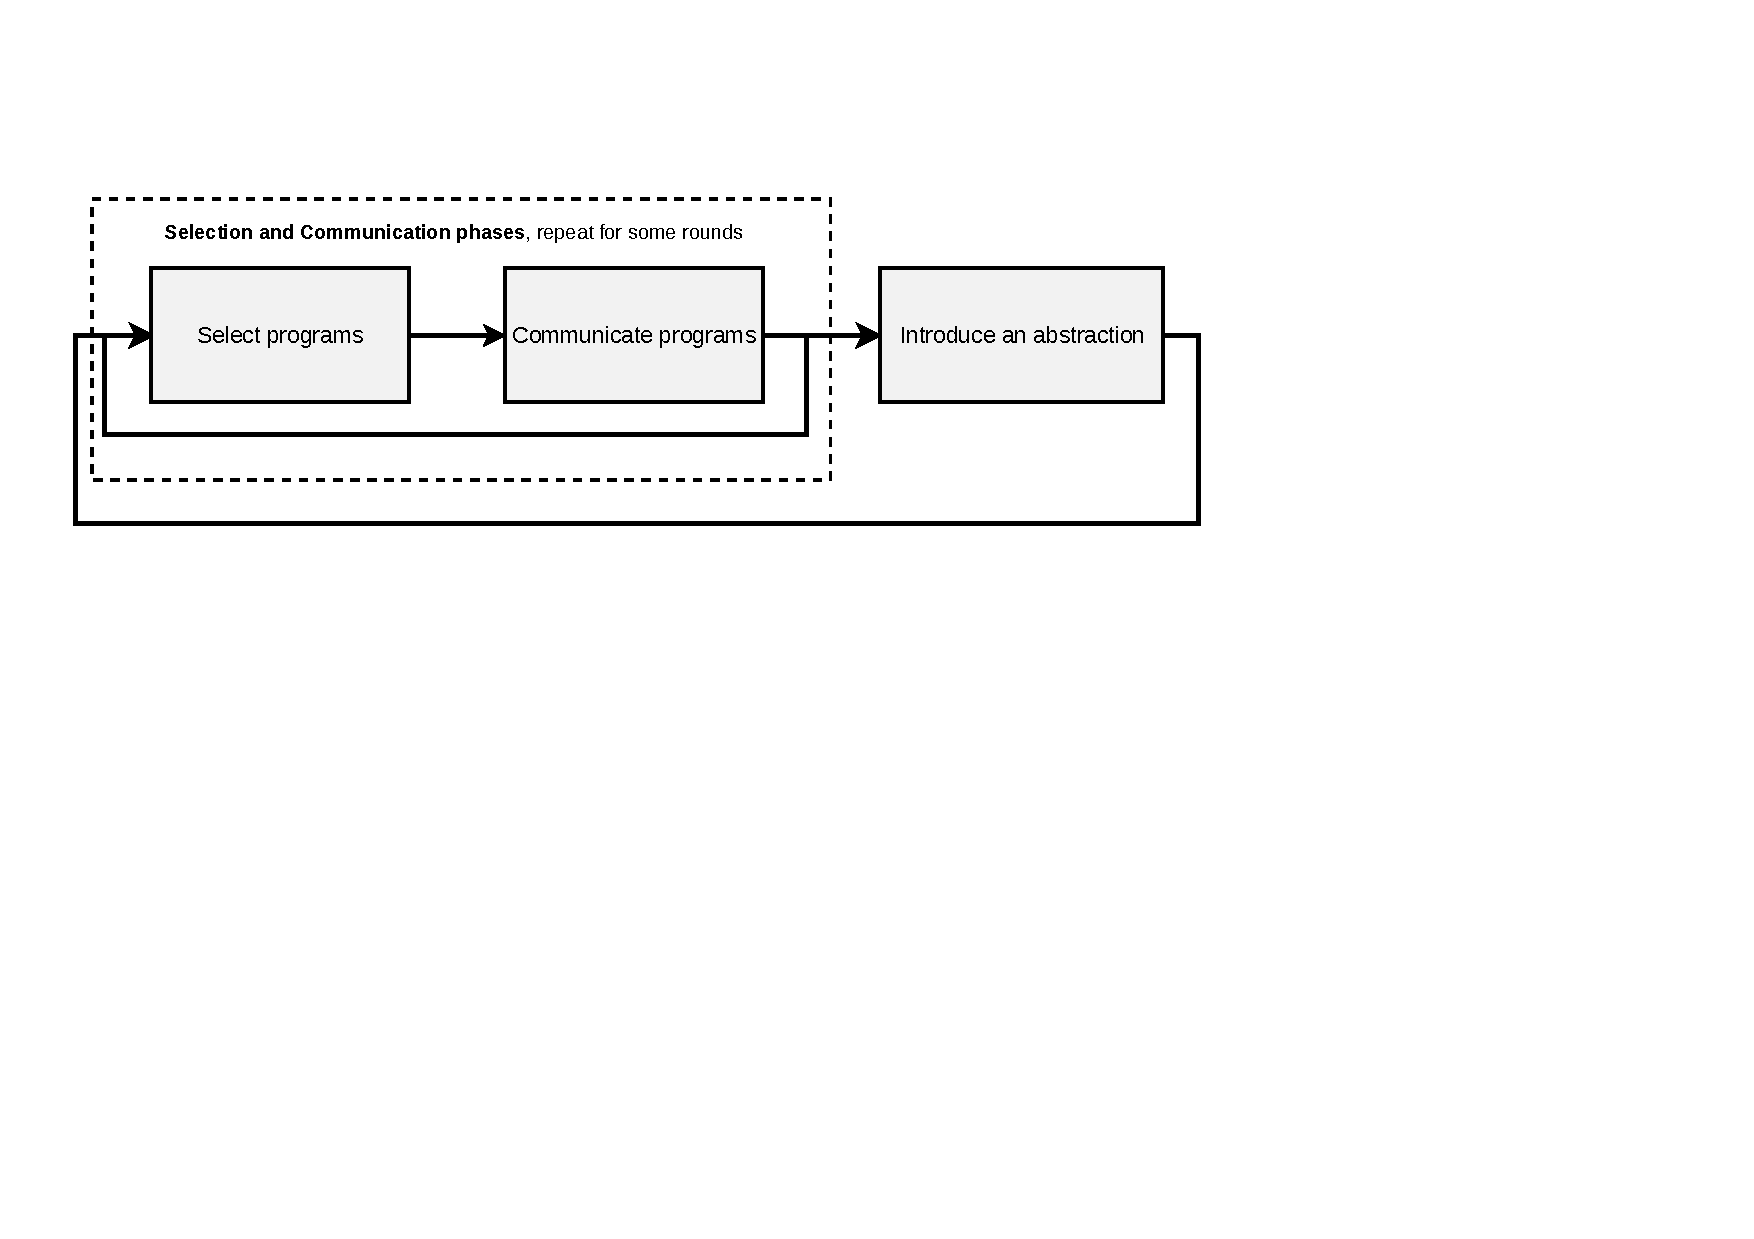
\includegraphics[width=0.9\textwidth,trim=35bp 342bp 265bp 95bp,clip]{images/Diagramma senza titolo.drawio (3).pdf}
    \caption{The three phases of PACE and their interaction during training. Selection chooses which program to communicate for each scene; Communication runs the neural signalling between speaker and listener; and Abstraction introduces a new reusable token into the vocabulary. Adapted from Figure 2 of Thomas et al.~\cite{thomas_pace_2025}.}
    \label{fig:pace-phases}
\end{figure}

The three phases interact as follows during training. The system starts with $\mathcal{A} = \{a_{\text{horiz}}, a_{\text{vert}}\}$ and one program per scene. Selection and Communication then run together for some number of epochs, during which the speaker's neural policy learns to communicate primitive actions and the bandit learns which programs work well. After enough epochs of Communication have accumulated, an Abstraction phase is triggered: the system adds one new abstraction to $\mathcal{A}$, extending the pool of programs available for each relevant scene. Selection and Communication then resume with the enlarged vocabulary, and the cycle repeats. The concrete training loop is described in Section~\ref{sec:pace-training-loop}.

\section{Selection: Choosing Which Program to Communicate}
\label{sec:pace-selection}

The Selection phase is the responsibility of a \textbf{contextual multi-armed bandit}. Its role is to decide, for each training scene, which program to hand off to the Communication phase.

At the start of training this decision is trivial: each scene has exactly one available program, written entirely in primitives, and that is what gets communicated. But as abstractions are introduced, a given scene may accumulate multiple programs of different lengths. Programs that use recently introduced abstractions are shorter, but they may also be less understood by the listener at that moment, since the listener has had less training exposure to those abstractions. Programs written entirely in primitives are longer, but the listener is guaranteed to interpret them correctly if it has already learned the two primitive tokens. The choice between the two is a classic exploration-exploitation trade-off, which is why PACE uses a bandit to handle it.

The bandit maintains a table of \textbf{Q-values}, one for each action $a \in \mathcal{A}$ in the current lexicon. The Q-value $Q(a)$ estimates how successfully action $a$ is currently being communicated: if the listener reliably interprets $a$ correctly, $Q(a)$ is close to 1; if not, $Q(a)$ is close to 0. The quality of a full program $p = [a_1, \ldots, a_\ell]$ is defined as the product of the Q-values of its actions, discounted by a factor $\gamma$:

\begin{equation}
    Q(p) = \prod_{i=1}^{|p|} \gamma \, Q(a_i).
    \label{eq:pace-program-value}
\end{equation}

Here $\gamma$ is a discount factor slightly smaller than 1 (in PACE, $\gamma = 0.99$). Two features of this formula are worth noting. First, the multiplicative form means that a program is only as strong as its weakest action: even a single low-Q action pulls the whole program's value down. Second, the discount $\gamma < 1$ compounds with program length: longer programs multiply more terms below 1 into the product, so their overall value is systematically smaller than that of shorter programs with equivalent per-action quality. This is how PACE encodes the pressure toward shorter programs, without needing an explicit length penalty in the loss.

Given the Q-values of all available programs for a scene, the bandit picks the program to communicate using an \textbf{epsilon-greedy} strategy: with probability $1 - \varepsilon$ it picks the program with the highest $Q(p)$, and with probability $\varepsilon$ it picks a program uniformly at random from those available. PACE uses $\varepsilon = 0.1$, meaning that 10\% of the time the bandit explores a suboptimal program to keep its Q-value estimates fresh.

After a program has been communicated (see Section~\ref{sec:pace-communication}), the bandit receives a reward for each action $a_i$ in the program: $r_i = 1$ if the listener interpreted $a_i$ correctly (i.e. reconstructed the correct next grid state), and $r_i = 0$ otherwise. The Q-value of each action is then updated using the standard incremental rule from Section~\ref{sec:bg-bandits}:

\begin{equation}
    Q(a_i) \leftarrow Q(a_i) + \alpha \, (r_i - Q(a_i)),
    \label{eq:pace-q-update}
\end{equation}

where $\alpha$ is the bandit learning rate (in PACE, $\alpha = 0.5$). When a new abstraction is introduced into $\mathcal{A}$ during an Abstraction phase (Section~\ref{sec:pace-abstraction}), its Q-value is initialised to $q_{\text{init}} = 0$. This pessimistic initialisation, discussed in the original paper~\cite{thomas_pace_2025}, prevents the bandit from forcing a brand-new abstraction into use before the listener has had the opportunity to interpret it.

\section{Communication: Signalling Actions to the Listener}
\label{sec:pace-communication}

The Communication phase runs the actual neural signalling between speaker and listener. Given a program $p$ selected by the bandit, the speaker and listener play a \textbf{one-step signalling game} for each action $a_i$ of the program.

Each such signalling game takes the form of a triple $(x_i, a_i, x_{i+1})$: the current grid state $x_i$ is transformed into the next grid state $x_{i+1}$ by applying action $a_i$. The speaker learns a neural \textbf{communication policy} $\pi_{\text{comm}}$ that maps the action $a_i$ to a discrete message:

\begin{equation}
    m_i = \pi_{\text{comm}}(a_i).
    \label{eq:pace-speaker}
\end{equation}

Similarly, the listener learns a neural \textbf{builder policy} $\pi_{\text{bldr}}$ that estimates the next grid state given the current state and the message:

\begin{equation}
    \widehat{x}_{i+1} = \pi_{\text{bldr}}(x_i, m_i).
    \label{eq:pace-listener}
\end{equation}

Both $\pi_{\text{comm}}$ and $\pi_{\text{bldr}}$ are implemented as fully connected neural networks. Since the message $m_i$ is discrete but the two policies must be trained end-to-end via gradient descent, PACE uses the Gumbel-softmax relaxation with the hard parameter~\cite{jang_categorical_2017}, which allows a discrete token to be sampled in the forward pass while a continuous relaxation is used in backpropagation. The two policies are jointly trained to minimise the binary cross-entropy loss between the target next state $x_{i+1}$ and the listener's prediction $\widehat{x}_{i+1}$:

\begin{equation}
    \mathcal{L}(\pi_{\text{comm}}, \pi_{\text{bldr}}) = \text{BCE}(x_{i+1}, \widehat{x}_{i+1}).
    \label{eq:pace-loss}
\end{equation}

Two implementation details of the Communication phase are worth flagging. The first is a positional encoding: along with each action $a_i$, PACE attaches information about the column at which the block is being dropped, which is passed to the listener alongside the state $x_i$ and the message $m_i$. Positional information is treated as pre-determined and does not need to be communicated: PACE's focus is on abstractions of shapes, not of positions. The second is a bias for \textit{positive signalling}~\cite{eccles_biases_2019} added to the speaker's loss, which encourages the messages the speaker produces to carry meaningful information about the action they represent, addressing a known failure mode in emergent communication where messages become uncorrelated with the underlying actions.

\section{Abstraction: Introducing New Reusable Tokens}
\label{sec:pace-abstraction}

The Abstraction phase introduces one new abstraction into the lexicon $\mathcal{A}$. It runs periodically, after a fixed number of Communication epochs have accumulated. Its role is to identify a sub-sequence of primitives (or of previously adopted abstractions) that is worth turning into a single reusable token.

The system starts by inspecting the current pool of programs across all training scenes, and enumerating all contiguous sub-sequences that appear in them. Each candidate sub-sequence $a_{\text{cand}}$ is scored according to an MDL-inspired criterion (Section~\ref{sec:bg-mdl}) that measures the expected reduction in program length that would result from adopting it. Formally, the criterion PACE uses is

\begin{equation}
    P(\mathcal{A} \cup \{a_{\text{cand}}\} \mid \{p_i\}_{i=1}^N) \propto \prod_{i=1}^N P(p_i \mid \mathcal{A} \cup \{a_{\text{cand}}\}),
    \label{eq:pace-abstraction-selection}
\end{equation}

where $\{p_i\}_{i=1}^N$ are the programs known so far and the right-hand side is defined as

\begin{equation}
    P(p_i \mid \mathcal{A} \cup \{a_{\text{cand}}\}) = \exp\bigl(-\text{MDL}(p_i \mid \mathcal{A} \cup \{a_{\text{cand}}\})\bigr).
    \label{eq:pace-mdl-def}
\end{equation}

Here $\text{MDL}(p_i \mid \mathcal{A} \cup \{a_{\text{cand}}\})$ is the shortest description length of program $p_i$ achievable using the extended lexicon, and the exponential converts shorter description lengths into higher probabilities. The candidate that maximises Equation~\ref{eq:pace-abstraction-selection} is the one whose introduction would compress the current programs the most in aggregate.

Once the winning candidate $a_{\text{cand}}$ is selected, it is added to the lexicon: $\mathcal{A} \leftarrow \mathcal{A} \cup \{a_{\text{cand}}\}$. Its Q-value is initialised to $q_{\text{init}} = 0$ as discussed in Section~\ref{sec:pace-selection}. For every training scene whose program contains at least one occurrence of the sub-sequence corresponding to $a_{\text{cand}}$, a new shorter program is generated by replacing that sub-sequence with the new abstraction token, and added to the pool of alternative programs available for that scene. The bandit is now free to select this shorter alternative from the next Communication phase onwards, subject to its exploration-exploitation trade-off. Figure~\ref{fig:pace-abstraction-cycle} illustrates this transition from primitive-only communication to a shorter abstraction-using program.

\begin{figure}[H]
    \centering
    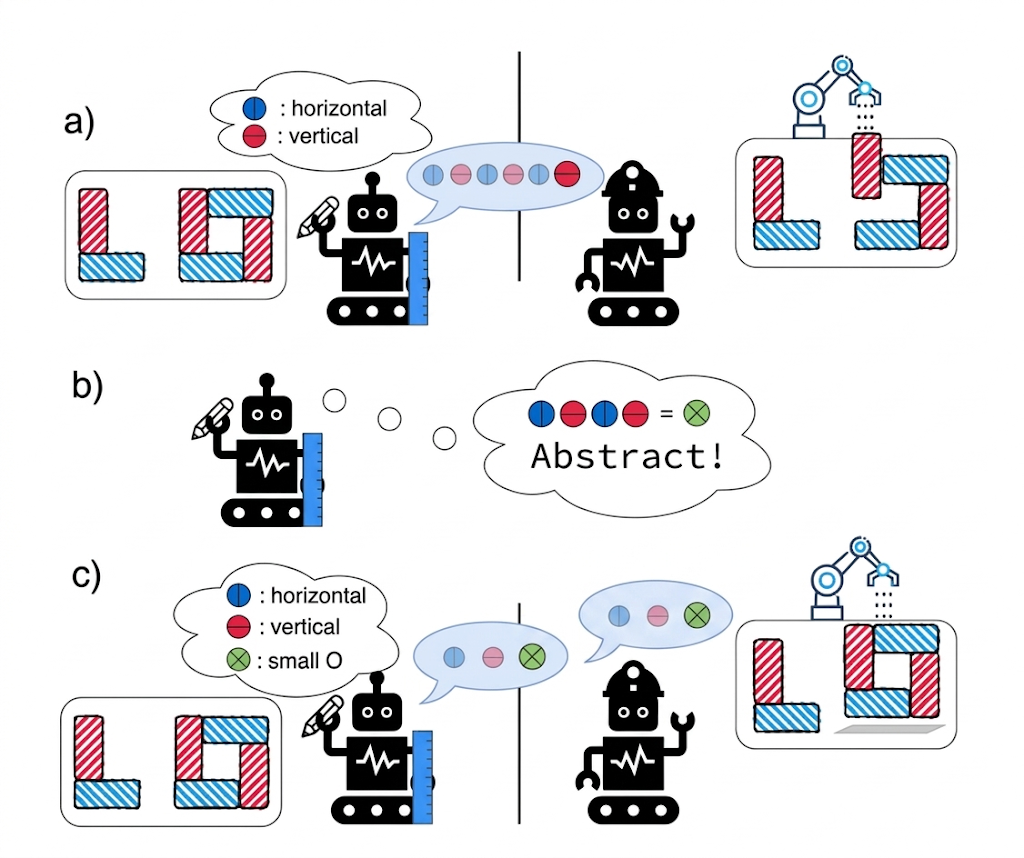
\includegraphics[width=0.85\textwidth]{images/figure_1_PACE.png}
    \caption{Illustration of the architect-builder game in PACE across three stages of a training cycle. In (a), the two agents communicate using only primitive tokens for horizontal and vertical blocks. In (b), the system introduces a new abstraction: a single token that represents a recurring sub-sequence of primitives. In (c), after a learning period, the same target scene can be described with a shorter program that uses the newly adopted abstraction. Recreated based on Figure~1 of Thomas et al.~\cite{thomas_pace_2025}.}
    \label{fig:pace-abstraction-cycle}
\end{figure}


To keep the number of alternative programs per scene manageable, PACE prunes each scene's pool to retain only the three programs with the highest Q-values before the next Abstraction phase. This prevents an exponential growth in program count that would otherwise result from stacking multiple rounds of abstraction introduction.

\section{The Training Loop}
\label{sec:pace-training-loop}

The training loop of PACE alternates between phases as follows. The system starts with $\mathcal{A} = \{a_{\text{horiz}}, a_{\text{vert}}\}$ and one primitive-only program per training scene. Two hyperparameters control the loop: the number of \textbf{Abstraction steps} $s$ and the number of \textbf{Communication epochs per step} $e$. PACE uses $s = 20$ and $e = 40$.

Each iteration of the outer loop begins with a Communication phase of $e = 40$ epochs. In each epoch, the training scenes are processed in mini-batches, and for each scene the bandit performs a Selection to pick which of the available programs to communicate. The scene is then broken into individual actions, and for each action the speaker-listener pair plays a one-step signalling game, produces a prediction of the next grid state, and receives a reconstruction loss that is backpropagated to update both the speaker's and the listener's neural parameters. The reward from the reconstruction is used to update the bandit's Q-values via Equation~\ref{eq:pace-q-update}. At the end of the 40 epochs, the neural agents have converged to a communication policy on the current vocabulary $\mathcal{A}$, and the bandit has an updated estimate of which programs work well.

An Abstraction phase then runs once at the end of the 40 epochs. A new abstraction is selected according to Equation~\ref{eq:pace-abstraction-selection}, added to $\mathcal{A}$, and used to generate shorter alternative programs for the relevant scenes. The next iteration of the outer loop then begins, with a new Communication phase of 40 epochs during which the neural agents adapt to the enlarged vocabulary.

After $s = 20$ iterations of this outer loop, training terminates. The trained agent is characterised by three components: the neural parameters of $\pi_{\text{comm}}$ and $\pi_{\text{bldr}}$, the abstraction tracker that lists the tokens adopted into $\mathcal{A}$ over the course of training, and the bandit state that records the Q-values of every abstraction ever proposed. These three components are all that Chapter~\ref{ch:rq3} needs to run the cross-pairing experiments.

\section{What This Thesis Extends}
\label{sec:pace-extensions}

The PACE architecture just described is used unchanged in this thesis, with two extensions. Both concern the experimental setup around PACE rather than the architecture itself.

The first extension is on the input side. The original PACE paper trains on a uniform distribution over the 930 training scenes: every scene appears with equal probability across training batches. In this thesis, we replace the uniform distribution with a family of Zipfian distributions parametrised by a concentration parameter $\alpha$, allowing us to move smoothly from the uniform case ($\alpha = 0$) to increasingly concentrated cases (up to $\alpha = 3$). The specifics of the construction are described in Section~\ref{sec:framework-shape-dataset}.

The second extension is a checkpointing and cross-pairing evaluation pipeline. When we pair the speaker of one training run with the listener of another, we load three checkpoint components from the speaker's original training: its neural parameters $\pi_{\text{comm}}$, its abstraction tracker (which defines the meaning of every token in its vocabulary), and its bandit state (which determines which programs it prefers to communicate). We then load the listener's neural parameters $\pi_{\text{bldr}}$ from a different training checkpoint. Communication-phase training then proceeds as in Section~\ref{sec:pace-communication}, with either only the listener adapting (in the frozen-speaker variant) or both adapting (in the unfrozen-speaker variant). The speaker's abstraction tracker and bandit state come from its original training and remain the reference against which the listener is expected to align. This pipeline is what enables the cross-population experiments of Chapter~\ref{ch:rq3}.

The neural architecture is otherwise unchanged from the original PACE paper: same fully connected speaker and listener with Gumbel-softmax head, same reconstruction loss, same positive-signalling bias. The symbolic subsystem is also unchanged: same MDL scoring rule, same proposal cadence, same shortlist size, and same epsilon-greedy bandit update. The purpose of these conservative choices is to isolate the effect of the input distribution from confounds introduced by architectural changes. Any pattern observed in the emergent language, in the divergence between populations, or in the cross-population communication should be attributable to the concentration parameter of the training input, not to a modification of the agents or the symbolic subsystem. The next chapter describes the experimental framework in which these extensions are put to work.